 % \chapter{Anhang}


% 1 Einleitung
% %%%%%%%%%%%%%%%%%%%%%%%%%%%%%%%%%%%%%%%%%%%%%%%%%%%%%%%%%%%%%%%%%%%%%%%%%%%%%

% \section{Einleitung}






% 2 Auswahl der Hardware
% %%%%%%%%%%%%%%%%%%%%%%%%%%%%%%%%%%%%%%%%%%%%%%%%%%%%%%%%%%%%%%%%%%%%%%%%%%%%%

% \section{Auswahl der Hardware}






% 3 System
% %%%%%%%%%%%%%%%%%%%%%%%%%%%%%%%%%%%%%%%%%%%%%%%%%%%%%%%%%%%%%%%%%%%%%%%%%%%%%

% \section{System}





% 4 Zynq
% %%%%%%%%%%%%%%%%%%%%%%%%%%%%%%%%%%%%%%%%%%%%%%%%%%%%%%%%%%%%%%%%%%%%%%%%%%%%%
\section{Zynq}

\subsection{Schema Zybo}
\label{anhang:schemaZybo}
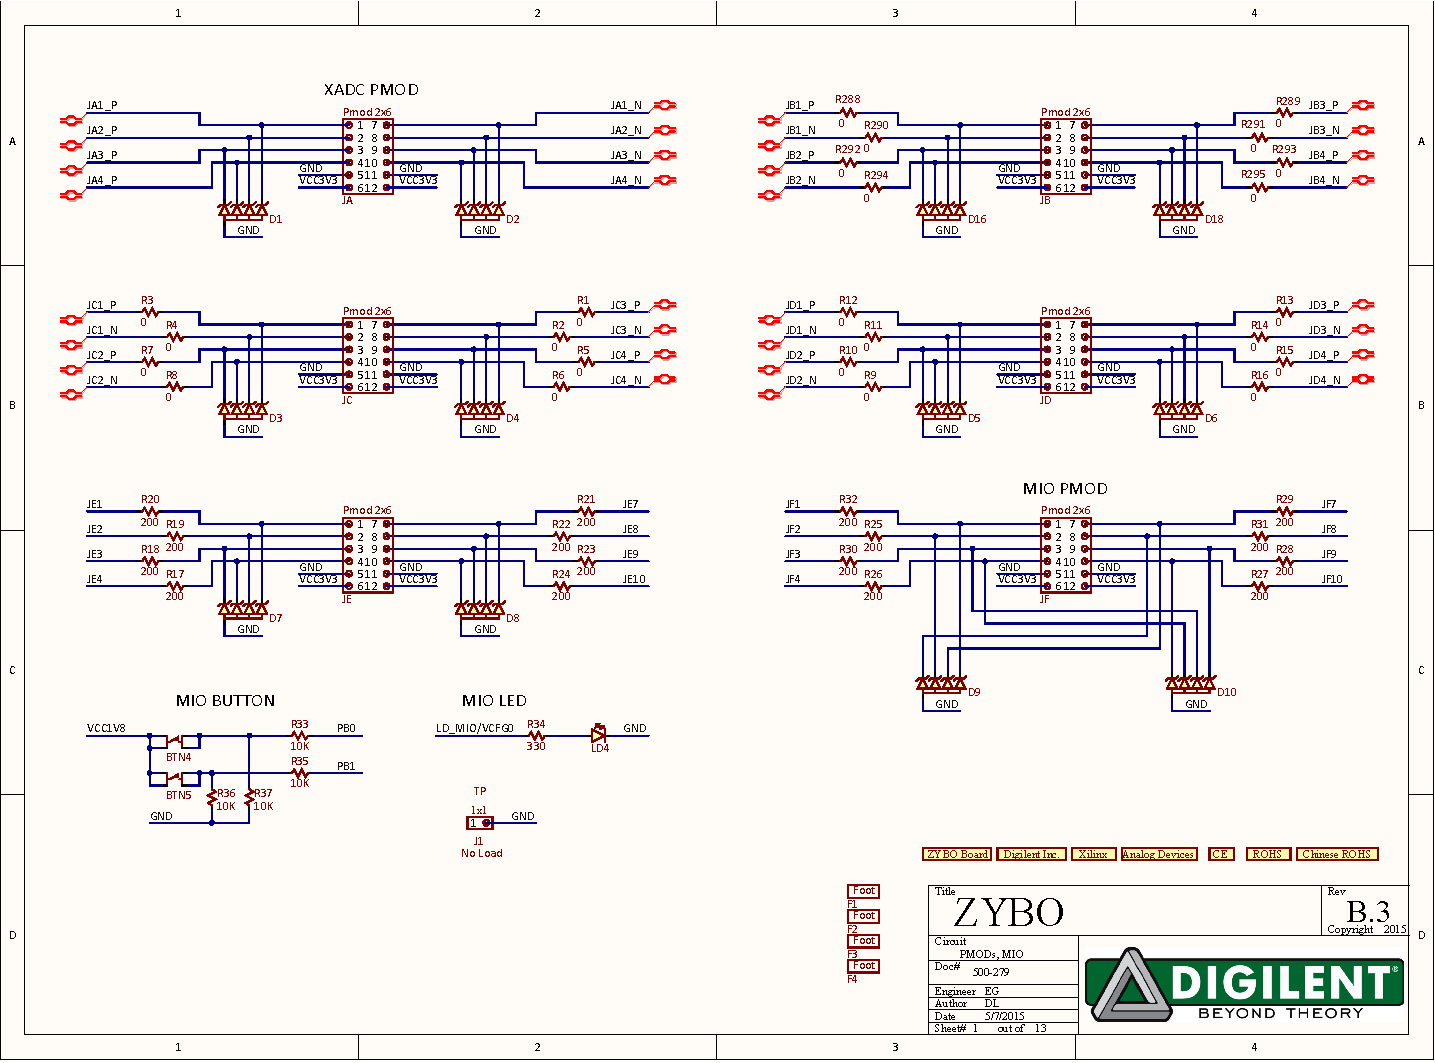
\includepdf[pages=-, landscape=true]{appendix/zybo_schematic.pdf}

% \label{anhang:zybo-ftdi.cfg-orig}
% \textit{zybo-ftdi.ocd original:}
% \lstset{language=tcl}
% \begin{lstlisting}
% #
% # ZYBO ft2232hq usbserial jtag
% #

% interface ftdi
% ftdi_device_desc "Digilent Adept USB Device"
% ftdi_vid_pid 0x0403 0x6010

% ftdi_layout_init 0x3088 0x1f8b
% #ftdi_layout_signal nTRST -data 0x1000 -oe 0x1000
% # 0x2000 is reset
% ftdi_layout_signal nSRST -data 0x3000 -oe 0x1000
% # green MIO7 LED
% ftdi_layout_signal LED -data 0x0010
% #ftdi_layout_signal LED -data 0x1000

% reset_config srst_pulls_trst
% \end{lstlisting}






% 5 openOCD
% %%%%%%%%%%%%%%%%%%%%%%%%%%%%%%%%%%%%%%%%%%%%%%%%%%%%%%%%%%%%%%%%%%%%%%%%%%%%%
\section{OpenOCD}

\subsection{zybo-ftdi.cfg angepasst:}
\label{anhang:zybo-ftdi.cfg}
\lstset{language=tcl}
\begin{lstlisting}
#
# FTDI2232 on Zybo
#
#  https://github.com/f32c/f32c/blob/master/rtl/proj/xilinx/zybo/xram_bram_hdmi_ise/ftdi-zybo.ocd 

interface ftdi
ftdi_device_desc "Digilent Adept USB Device"
ftdi_vid_pid 0x0403 0x6010

#ftdi_layout_init data direction
ftdi_layout_init 0x3088 0x1f8b

ftdi_layout_signal nSRST -data 0x3000 -oe 0x3000

# green MIO7 LED
ftdi_layout_signal LED -data 0x0010

reset_config srst_only
adapter_nsrst_delay 40
\end{lstlisting}


\subsection{zybo.cfg angepasst:}
\label{anhang:zybo.cfg}
\lstset{language=tcl}
\begin{lstlisting}
#
# ZYBO board
#
# https://github.com/emard/wifi_jtag/blob/master/openocd/scripts/board/zybo.cfg 

set _CHIPNAME zynq
set _TARGETNAME $_CHIPNAME.cpu

jtag newtap chip tap -irlen 6 -ircapture 0x1 -irmask 0x03 \
    -expected-id 0x23727093 \
    -expected-id 0x03727093 \
    -expected-id 0x13722093

jtag newtap $_CHIPNAME dap -irlen 4 -ircapture 0x1 -irmask 0xf -expected-id 0x4ba00477

target create ${_TARGETNAME}0 cortex_a -chain-position $_CHIPNAME.dap \
    -coreid 0 -dbgbase 0x80090000
target create ${_TARGETNAME}1 cortex_a -chain-position $_CHIPNAME.dap \
    -coreid 1 -dbgbase 0x80092000
target smp ${_TARGETNAME}0 ${_TARGETNAME}1

adapter_khz 1000

${_TARGETNAME}0 configure -event reset-assert-post "cortex_a dbginit"
${_TARGETNAME}1 configure -event reset-assert-post "cortex_a dbginit"

script ps7_init_modified.tcl

# http://openocd.org/doc/html/CPU-Configuration.html#targetevents
${_TARGETNAME}0 configure -event reset-init {
	echo "Running reset init script for Zybo"
	# Reset script for AT91EB40a
#	map_OCM_low
	initPS
}


init
scan_chain
halt

#map_OCM_low
#initPS
\end{lstlisting}


\label{anhang:zynq_7000.cfg}




\subsection{Xilinx SDK Log:}
\label{anhang:SDKLog}
\lstset{language=plain}
\begin{lstlisting}
14:26:34 INFO	: Disconnected from the channel tcfchan#2.
14:26:36 INFO	: 'targets -set -filter {jtag_cable_name =~ "Digilent Zybo 210279573773A" && level==0} -index 1' command is executed.
14:26:36 INFO	: 'fpga -state' command is executed.
14:26:36 INFO	: Connected to target on host '127.0.0.1' and port '3121'.
14:26:36 INFO	: Jtag cable 'Digilent Zybo 210279573773A' is selected.
14:26:36 INFO	: 'jtag frequency' command is executed.
14:26:36 INFO	: Sourcing of 'D:/Vivado/01_gettingStarted/01_gettingStarted.sdk/design_1_wrapper_hw_platform_0/ps7_init.tcl' is done.
14:26:36 INFO	: Context for 'APU' is selected.
14:26:38 INFO	: Hardware design information is loaded from 'D:/Vivado/01_gettingStarted/01_gettingStarted.sdk/design_1_wrapper_hw_platform_0/system.hdf'.
14:26:38 INFO	: 'configparams force-mem-access 1' command is executed.
14:26:38 INFO	: Context for 'APU' is selected.
14:26:38 INFO	: 'stop' command is executed.
14:26:38 INFO	: 'ps7_init' command is executed.
14:26:38 INFO	: 'ps7_post_config' command is executed.
14:26:38 INFO	: Context for processor 'ps7_cortexa9_0' is selected.
14:26:38 INFO	: Processor reset is completed for 'ps7_cortexa9_0'.
14:26:38 INFO	: Context for processor 'ps7_cortexa9_0' is selected.
14:26:39 INFO	: The application 'D:/Vivado/01_gettingStarted/01_gettingStarted.sdk/01_gettingStarted_ApplicationProject/Debug/01_gettingStarted_ApplicationProject.elf' is downloaded to processor 'ps7_cortexa9_0'.
14:26:39 INFO	: 'configparams force-mem-access 0' command is executed.
14:26:39 INFO	: ----------------XSDB Script----------------
connect -url tcp:127.0.0.1:3121
source D:/Vivado/01_gettingStarted/01_gettingStarted.sdk/design_1_wrapper_hw_platform_0/ps7_init.tcl
targets -set -nocase -filter {name =~"APU*" && jtag_cable_name =~ "Digilent Zybo 210279573773A"} -index 0
loadhw -hw D:/Vivado/01_gettingStarted/01_gettingStarted.sdk/design_1_wrapper_hw_platform_0/system.hdf -mem-ranges [list {0x40000000 0xbfffffff}]
configparams force-mem-access 1
targets -set -nocase -filter {name =~"APU*" && jtag_cable_name =~ "Digilent Zybo 210279573773A"} -index 0
stop
ps7_init
ps7_post_config
targets -set -nocase -filter {name =~ "ARM*#0" && jtag_cable_name =~ "Digilent Zybo 210279573773A"} -index 0
rst -processor
targets -set -nocase -filter {name =~ "ARM*#0" && jtag_cable_name =~ "Digilent Zybo 210279573773A"} -index 0
dow D:/Vivado/01_gettingStarted/01_gettingStarted.sdk/01_gettingStarted_ApplicationProject/Debug/01_gettingStarted_ApplicationProject.elf
configparams force-mem-access 0
----------------End of Script----------------

14:26:39 INFO	: Memory regions updated for context APU
14:26:39 INFO	: Context for processor 'ps7_cortexa9_0' is selected.
14:26:39 INFO	: 'con' command is executed.
14:26:39 INFO	: ----------------XSDB Script (After Launch)----------------
targets -set -nocase -filter {name =~ "ARM*#0" && jtag_cable_name =~ "Digilent Zybo 210279573773A"} -index 0
con
----------------End of Script----------------

14:26:39 INFO	: Launch script is exported to file 'D:\Vivado\01_gettingStarted\01_gettingStarted.sdk\.sdk\launch_scripts\xilinx_c-c++_application_(system_debugger)\system_debugger_using_debug_01_gettingstarted_applicationproject.elf_on_local.tcl'
\end{lstlisting}


\subsection{system\_debugger\_using\_debug\_01\_gettingstarted\\\_applicationproject.elf\_on\_local.tcl:}
\label{anhang:elf_on_local.tcl}
\lstset{language=plain}
\begin{lstlisting}
connect -url tcp:127.0.0.1:3121
source D:/Vivado/01_gettingStarted/01_gettingStarted.sdk/design_1_wrapper_hw_platform_0/ps7_init.tcl
targets -set -nocase -filter {name =~"APU*" && jtag_cable_name =~ "Digilent Zybo 210279573773A"} -index 0
loadhw -hw D:/Vivado/01_gettingStarted/01_gettingStarted.sdk/design_1_wrapper_hw_platform_0/system.hdf -mem-ranges [list {0x40000000 0xbfffffff}]
configparams force-mem-access 1
targets -set -nocase -filter {name =~"APU*" && jtag_cable_name =~ "Digilent Zybo 210279573773A"} -index 0
stop
ps7_init
ps7_post_config
targets -set -nocase -filter {name =~ "ARM*#0" && jtag_cable_name =~ "Digilent Zybo 210279573773A"} -index 0
rst -processor
targets -set -nocase -filter {name =~ "ARM*#0" && jtag_cable_name =~ "Digilent Zybo 210279573773A"} -index 0
dow D:/Vivado/01_gettingStarted/01_gettingStarted.sdk/01_gettingStarted_ApplicationProject/Debug/01_gettingStarted_ApplicationProject.elf
configparams force-mem-access 0
targets -set -nocase -filter {name =~ "ARM*#0" && jtag_cable_name =~ "Digilent Zybo 210279573773A"} -index 0
con
\end{lstlisting}


\subsection{CLI-OpenOCD-Toolchain}
\label{anhang:CLI-OpenOCD-Toolchain}
\lstset{language=java}
\begin{lstlisting}
#deep-1

meta {
	version = "2018-02-28";
	description = "Programmer description file for use with OpenOCD";
}

programmer openOCD {
	description = "OpenOCD";
	pluginid = "ch.ntb.inf.openOCDInterface";
	classname = "ch.ntb.inf.openOCDInterface.OpenOCD";
}
\end{lstlisting}






% 6 Das ELF-Dateiformat
% %%%%%%%%%%%%%%%%%%%%%%%%%%%%%%%%%%%%%%%%%%%%%%%%%%%%%%%%%%%%%%%%%%%%%%%%%%%%%
\section{Das ELF-Dateiformat}
\label{anhang:DasELF-Dateiformat}
\subsection{loop.java:}
\label{anhang:loop.java}
\lstset{language=java}
\begin{lstlisting}
static void reset() {



	US.PUTGPR(SP, stackBase + stackSize - 4);	// set stack pointer
	
	int x00 = 0;
	int x01 = 1;
	int x02 = 2;
	
	x00++;
	x01++;
	x02++;
	
	int x100 = 100;
	for(int i=0; i<10; i++){
		x100 += 10;
   }
		
	x100++;
	x100++;
	x100++;
	x100++;
	x100++;

	US.ASM("b -8"); // stop here
}
\end{lstlisting}


\subsection{stabs.include:}
\label{anhang:stabs.include}
\lstset{language={[x86masm]Assembler}}
\begin{lstlisting}
# non-stab symbol types
.set N_UNDF,		0x0
.set N_EXT,			0x1
.set N_ABS,			0x2
.set N_TEXT,		0x4
.set N_DATA,		0x6
.set N_BSS,			0x8
.set N_FN_SEQ,		0x0c
.set N_INDR,		0x0a
.set N_COMM,		0x12
.set N_SETA,		0x14
.set N_SETT,		0x16
.set N_SETD,		0x18
.set N_SETB,		0x1a
.set N_SETV,		0x1c
.set N_WARNING,		0x1e
.set N_FN,			0x1f

# stab symbol types
.set N_GSYM,		0x20
.set N_FNAME,		0x22
.set N_FUN,			0x24
.set N_STSYM,		0x26
.set N_LCSYM,		0x28
.set N_MAIN,		0x2a
.set N_ROSYM,		0x2c
.set N_PC,			0x30
.set N_NSYMS,		0x32
.set N_NOMAP,		0x34
.set N_MAC_DEFINE,	0x36
.set N_OBJ,			0x38
.set N_MAC_UNDEF,	0x3a
.set N_OPT,			0x3c
.set N_RSYM,		0x40
.set N_M2C,			0x42
.set N_SLINE,		0x44
.set N_DSLINE,		0x46
.set N_BSLINE,		0x48
.set N_BROWS,		0x48
.set N_DEFD,		0x4a
.set N_FLINE,		0x4c
.set N_EHDECL,		0x50
.set N_MOD2,		0x50
.set N_CATCH,		0x54
.set N_SSYM,		0x60
.set N_ENDM,		0x62
#.set N_SO,			0x100
.set N_SO,			0x64
.set N_LSYM,		0x80
.set N_BINCL,		0x82
.set N_SOL,			0x84
.set N_PSYM,		0xa0
.set N_EINCL,		0xa2
.set N_ENTRY,		0xa4
.set N_LBRAC,		0xc0
.set N_EXCL,		0xc2
.set N_SCOPE,		0xc4
.set N_RBRAC,		0xe0
.set N_BCOMM,		0xe2
.set N_ECOMM,		0xe4
.set N_ECOML,		0xe8
.set N_WITH,		0xea
.set N_NBTEXT,		0xf0
.set N_NBDATA,		0xf2
.set N_NBBSS,		0xf4
.set N_NBSTS,		0xf6
.set N_NBLCS,		0xf8
\end{lstlisting}



\subsection{loopExample.c}
\label{anhang:loopExample.c}
\lstset{language=c}
\begin{lstlisting}
int global = 111;


int c_entry() {
	int x00 = 0;
	int x01 = 10;
	int x02 = 20;
	x00++;
	x01++;
	x02++;
	register int s=1;
	float float0=1.1;
	int int0 = 10;
	for(int i=0; i<=2; i++) {
		int0=int0+10;
	}
	int0 = int0 + s;
	int0 = int0 + s;
	int0 = int0 + s;
	int0 = int0 + s;
	
	while(1);
  return 0;
}
\end{lstlisting}


\subsection{make\_loopExample.ps1}
\label{anhang:make_loopExample.ps1}
\lstset{language=sh}
\begin{lstlisting}
# Add the path for the GNU Arm Embedded Toolchain to the 'Env:Path' variable
$Env:Path += ";D:\GNUArmEmbeddedToolchain\7-2018-q2-update\bin"

# Change to directory containing the program
cd M:\MA\stabs\cExample


# Compile the C test program with automatic generated stabs
#   * -c      compile and assemble, but do not link.
#   * -O0     no optimization
#   * -march=armv7-a    compile for architecture armv7 
#   * -g      compile with debugsymbols
#   * -gstabs compile with stabs debug symbols
arm-none-eabi-gcc -c -march=armv7-a -O0 -g -gstabs loopExample.c -o loopExample.o

# Disassemble object file again
#   * --disassemble     : disassemble the executable code section
#   * --disassemble     : include all STABS informations
arm-none-eabi-objdump -d  -G  loopExample.o > loopExample.Sd



# Build for host
gcc -std=c99 -g loopExample.host.c -o loopExample.host.a
\end{lstlisting}



\subsection{loopExample.Sd}
\label{anhang:loopExample.Sd}
\lstset{language=plain}
\begin{lstlisting}

loopExample.o:     file format elf32-littlearm

Contents of .stab section:

Symnum n_type n_othr n_desc n_value  n_strx String

-1     HdrSym 0      84     000007e4 1     
0      SO     0      2      00000000 15     loopExample.c
1      OPT    0      0      00000000 29     gcc2_compiled.
2      LSYM   0      0      00000000 44     int:t(0,1)=r(0,1);-2147483648;2147483647;
3      LSYM   0      0      00000000 86     char:t(0,2)=r(0,2);0;255;
4      LSYM   0      0      00000000 112    long int:t(0,3)=r(0,3);-2147483648;2147483647;
5      LSYM   0      0      00000000 159    unsigned int:t(0,4)=r(0,4);0;4294967295;
6      LSYM   0      0      00000000 200    long unsigned int:t(0,5)=r(0,5);0;4294967295;
7      LSYM   0      0      00000000 246    __int128:t(0,6)=r(0,6);0;-1;
8      LSYM   0      0      00000000 275    __int128 unsigned:t(0,7)=r(0,7);0;-1;
9      LSYM   0      0      00000000 313    long long int:t(0,8)=r(0,8);-0;4294967295;
10     LSYM   0      0      00000000 356    long long unsigned int:t(0,9)=r(0,9);0;-1;
11     LSYM   0      0      00000000 399    short int:t(0,10)=r(0,10);-32768;32767;
12     LSYM   0      0      00000000 439    short unsigned int:t(0,11)=r(0,11);0;65535;
13     LSYM   0      0      00000000 483    signed char:t(0,12)=r(0,12);-128;127;
14     LSYM   0      0      00000000 521    unsigned char:t(0,13)=r(0,13);0;255;
15     LSYM   0      0      00000000 558    float:t(0,14)=r(0,1);4;0;
16     LSYM   0      0      00000000 584    double:t(0,15)=r(0,1);8;0;
17     LSYM   0      0      00000000 611    long double:t(0,16)=r(0,1);8;0;
18     LSYM   0      0      00000000 643    short _Fract:t(0,17)=r(0,1);1;0;
19     LSYM   0      0      00000000 676    _Fract:t(0,18)=r(0,1);2;0;
20     LSYM   0      0      00000000 703    long _Fract:t(0,19)=r(0,1);4;0;
21     LSYM   0      0      00000000 735    long long _Fract:t(0,20)=r(0,1);8;0;
22     LSYM   0      0      00000000 772    unsigned short _Fract:t(0,21)=r(0,1);1;0;
23     LSYM   0      0      00000000 814    unsigned _Fract:t(0,22)=r(0,1);2;0;
24     LSYM   0      0      00000000 850    unsigned long _Fract:t(0,23)=r(0,1);4;0;
25     LSYM   0      0      00000000 891    unsigned long long _Fract:t(0,24)=r(0,1);8;0;
26     LSYM   0      0      00000000 937    _Sat short _Fract:t(0,25)=r(0,1);1;0;
27     LSYM   0      0      00000000 975    _Sat _Fract:t(0,26)=r(0,1);2;0;
28     LSYM   0      0      00000000 1007   _Sat long _Fract:t(0,27)=r(0,1);4;0;
29     LSYM   0      0      00000000 1044   _Sat long long _Fract:t(0,28)=r(0,1);8;0;
30     LSYM   0      0      00000000 1086   _Sat unsigned short _Fract:t(0,29)=r(0,1);1;0;
31     LSYM   0      0      00000000 1133   _Sat unsigned _Fract:t(0,30)=r(0,1);2;0;
32     LSYM   0      0      00000000 1174   _Sat unsigned long _Fract:t(0,31)=r(0,1);4;0;
33     LSYM   0      0      00000000 1220   _Sat unsigned long long _Fract:t(0,32)=r(0,1);8;0;
34     LSYM   0      0      00000000 1271   short _Accum:t(0,33)=r(0,1);2;0;
35     LSYM   0      0      00000000 1304   _Accum:t(0,34)=r(0,1);4;0;
36     LSYM   0      0      00000000 1331   long _Accum:t(0,35)=r(0,1);8;0;
37     LSYM   0      0      00000000 1363   long long _Accum:t(0,36)=r(0,1);8;0;
38     LSYM   0      0      00000000 1400   unsigned short _Accum:t(0,37)=r(0,1);2;0;
39     LSYM   0      0      00000000 1442   unsigned _Accum:t(0,38)=r(0,1);4;0;
40     LSYM   0      0      00000000 1478   unsigned long _Accum:t(0,39)=r(0,1);8;0;
41     LSYM   0      0      00000000 1519   unsigned long long _Accum:t(0,40)=r(0,1);8;0;
42     LSYM   0      0      00000000 1565   _Sat short _Accum:t(0,41)=r(0,1);2;0;
43     LSYM   0      0      00000000 1603   _Sat _Accum:t(0,42)=r(0,1);4;0;
44     LSYM   0      0      00000000 1635   _Sat long _Accum:t(0,43)=r(0,1);8;0;
45     LSYM   0      0      00000000 1672   _Sat long long _Accum:t(0,44)=r(0,1);8;0;
46     LSYM   0      0      00000000 1714   _Sat unsigned short _Accum:t(0,45)=r(0,1);2;0;
47     LSYM   0      0      00000000 1761   _Sat unsigned _Accum:t(0,46)=r(0,1);4;0;
48     LSYM   0      0      00000000 1802   _Sat unsigned long _Accum:t(0,47)=r(0,1);8;0;
49     LSYM   0      0      00000000 1848   _Sat unsigned long long _Accum:t(0,48)=r(0,1);8;0;
50     LSYM   0      0      00000000 1899   void:t(0,49)=(0,49)
51     GSYM   0      0      00000000 1919   global:G(0,1)
52     FUN    0      0      00000000 1933   c_entry:F(0,1)
53     SLINE  0      4      00000000 0      
54     SLINE  0      5      0000000c 0      
55     SLINE  0      6      00000014 0      
56     SLINE  0      7      0000001c 0      
57     SLINE  0      8      00000024 0      
58     SLINE  0      9      00000030 0      
59     SLINE  0      10     0000003c 0      
60     SLINE  0      11     00000048 0      
61     SLINE  0      12     0000004c 0      
62     SLINE  0      13     00000058 0      
63     SLINE  0      14     00000060 0      
64     SLINE  0      15     0000006c 0      
65     SLINE  0      14     00000078 0      
66     SLINE  0      14     00000084 0      
67     SLINE  0      17     00000090 0      
68     SLINE  0      18     0000009c 0      
69     SLINE  0      19     000000a8 0      
70     SLINE  0      20     000000b4 0      
71     SLINE  0      22     000000c0 0      
72     LSYM   0      0      fffffff0 1948   x00:(0,1)
73     LSYM   0      0      ffffffec 1958   x01:(0,1)
74     LSYM   0      0      ffffffe8 1968   x02:(0,1)
75     RSYM   0      0      00000004 1978   s:r(0,1)
76     LSYM   0      0      ffffffe4 1987   float0:(0,14)
77     LSYM   0      0      fffffff8 2001   int0:(0,1)
78     LBRAC  0      0      00000000 0      
79     LSYM   0      0      fffffff4 2012   i:(0,1)
80     LBRAC  0      0      00000060 0      
81     RBRAC  0      0      00000090 0      
82     RBRAC  0      0      000000c4 0      
83     SO     0      0      000000c4 0      


Disassembly of section .text:

00000000 <c_entry>:
   0:	e92d0810 	push	{r4, fp}
   4:	e28db004 	add	fp, sp, #4
   8:	e24dd018 	sub	sp, sp, #24
   c:	e3a03000 	mov	r3, #0
  10:	e50b3010 	str	r3, [fp, #-16]
  14:	e3a0300a 	mov	r3, #10
  18:	e50b3014 	str	r3, [fp, #-20]	; 0xffffffec
  1c:	e3a03014 	mov	r3, #20
  20:	e50b3018 	str	r3, [fp, #-24]	; 0xffffffe8
  24:	e51b3010 	ldr	r3, [fp, #-16]
  28:	e2833001 	add	r3, r3, #1
  2c:	e50b3010 	str	r3, [fp, #-16]
  30:	e51b3014 	ldr	r3, [fp, #-20]	; 0xffffffec
  34:	e2833001 	add	r3, r3, #1
  38:	e50b3014 	str	r3, [fp, #-20]	; 0xffffffec
  3c:	e51b3018 	ldr	r3, [fp, #-24]	; 0xffffffe8
  40:	e2833001 	add	r3, r3, #1
  44:	e50b3018 	str	r3, [fp, #-24]	; 0xffffffe8
  48:	e3a04001 	mov	r4, #1
  4c:	e30c3ccd 	movw	r3, #52429	; 0xcccd
  50:	e3433f8c 	movt	r3, #16268	; 0x3f8c
  54:	e50b301c 	str	r3, [fp, #-28]	; 0xffffffe4
  58:	e3a0300a 	mov	r3, #10
  5c:	e50b3008 	str	r3, [fp, #-8]
  60:	e3a03000 	mov	r3, #0
  64:	e50b300c 	str	r3, [fp, #-12]
  68:	ea000005 	b	84 <c_entry+0x84>
  6c:	e51b3008 	ldr	r3, [fp, #-8]
  70:	e283300a 	add	r3, r3, #10
  74:	e50b3008 	str	r3, [fp, #-8]
  78:	e51b300c 	ldr	r3, [fp, #-12]
  7c:	e2833001 	add	r3, r3, #1
  80:	e50b300c 	str	r3, [fp, #-12]
  84:	e51b300c 	ldr	r3, [fp, #-12]
  88:	e3530002 	cmp	r3, #2
  8c:	dafffff6 	ble	6c <c_entry+0x6c>
  90:	e51b3008 	ldr	r3, [fp, #-8]
  94:	e0833004 	add	r3, r3, r4
  98:	e50b3008 	str	r3, [fp, #-8]
  9c:	e51b3008 	ldr	r3, [fp, #-8]
  a0:	e0833004 	add	r3, r3, r4
  a4:	e50b3008 	str	r3, [fp, #-8]
  a8:	e51b3008 	ldr	r3, [fp, #-8]
  ac:	e0833004 	add	r3, r3, r4
  b0:	e50b3008 	str	r3, [fp, #-8]
  b4:	e51b3008 	ldr	r3, [fp, #-8]
  b8:	e0833004 	add	r3, r3, r4
  bc:	e50b3008 	str	r3, [fp, #-8]
  c0:	eafffffe 	b	c0 <c_entry+0xc0>
\end{lstlisting}





\subsection{Reset.Java:}
\label{anhang:reset.java}
\lstset{language=java}
\begin{lstlisting}
/*
 * Copyright 2011 - 2013 NTB University of Applied Sciences in Technology
 * Buchs, Switzerland, http://www.ntb.ch/inf
 * 
 * Licensed under the Apache License, Version 2.0 (the "License");
 * you may not use this file except in compliance with the License.
 * You may obtain a copy of the License at
 * 
 * http://www.apache.org/licenses/LICENSE-2.0
 *   
 * Unless required by applicable law or agreed to in writing, software
 * distributed under the License is distributed on an "AS IS" BASIS,
 * WITHOUT WARRANTIES OR CONDITIONS OF ANY KIND, either express or implied.
 * See the License for the specific language governing permissions and
 * limitations under the License.
 * 
 */

package ch.ntb.inf.deep.runtime.zynq7000;
import ch.ntb.inf.deep.runtime.IdeepCompilerConstants;
import ch.ntb.inf.deep.runtime.arm32.Iarm32;
import ch.ntb.inf.deep.runtime.arm32.ARMException;
import ch.ntb.inf.deep.unsafe.US;

/* changes:
 * 13.05.16	NTB/Urs Graf	creation
 */
/**
 * The class for the ARM reset exception.
 * The stack pointer will be initialized and the program counter will be
 * set to the beginning of the class initializer of the kernel.
 * 
 * @author Urs Graf
 */
class Reset extends ARMException implements Iarm32, Izybo7000, IdeepCompilerConstants {
//	static int g = 5555;
	
	static void reset() {
		int stackOffset = US.GET4(sysTabBaseAddr + stStackOffset);
		int stackBase = US.GET4(sysTabBaseAddr + stackOffset + 4);
		int stackSize = US.GET4(sysTabBaseAddr + stackOffset + 8);
		US.PUTGPR(SP, stackBase + stackSize - 4);	// set stack pointer
		
		int x00 = 0;
		int x01 = 10;
		int x02 = 20;
		x00++;
		x01++;
		x02++;
		
		int x100 = 100;
		for(int i=0; i<10; i++){
            x100 += 10;
       }
		
		x100++;
		x100++;
		x100++;
		x100++;
		x100++;

		US.ASM("b -8"); // stop here

	}	
}
\end{lstlisting}




\subsection{loopMachineCode.txt:}
\label{anhang:loopMachineCode.txt}
\lstset{language=plain}
\begin{lstlisting}
Code for Method: ch/ntb/inf/deep/runtime/zynq7000/Reset.reset()V
	E3010004	[0x0]	movw R0, #4100
	E4101000	[0x4]	ldr R1, [R0], #-0
	E2810D40	[0x8]	add R0, R1, #4096
	E2802004	[0xc]	add R2, R0, #4
	E4120000	[0x10]	ldr R0, [R2], #-0
	E2812D40	[0x14]	add R2, R1, #4096
	E2821008	[0x18]	add R1, R2, #8
	E4112000	[0x1c]	ldr R2, [R1], #-0
	E0801002	[0x20]	add R1, R0, R2, 0
	E2410004	[0x24]	sub R0, R1, #4
	E1A0D000	[0x28]	mov R13, R0
	E3000000	[0x2c]	movw R0, #0
	E300100A	[0x30]	movw R1, #10
	E3002014	[0x34]	movw R2, #20
	E2803001	[0x38]	add R3, R0, #1
	E2810001	[0x3c]	add R0, R1, #1
	E2820001	[0x40]	add R0, R2, #1
	E3000064	[0x44]	movw R0, #100
	E3001000	[0x48]	movw R1, #0
	EA000001	[0x4c]	b 12, [0x58]	
	E280000A	[0x50]	add R0, R0, #10
	E2811001	[0x54]	add R1, R1, #1
	E351000A	[0x58]	cmp R1, #10
	BAFFFFFB	[0x5c]	b if less -12, [0x50]	
	E2801001	[0x60]	add R1, R0, #1
	E2810001	[0x64]	add R0, R1, #1
	E2801001	[0x68]	add R1, R0, #1
	E2810001	[0x6c]	add R0, R1, #1
	E2801001	[0x70]	add R1, R0, #1
	EAFFFFFE	[0x74]	b 0, [0x74]	
\end{lstlisting}


\subsection{loop.S:}
\label{anhang:loop.S}
\lstset{language={[x86masm]Assembler}}
\begin{lstlisting}
.global _start

.org 0x000000
.text
Ltext0:

_start:
_reset:
c_entry:
movw R13, #1024

movw R0, #0
movw R1, #10
movw R2, #20
add R3, R0, #1
add R0, R1, #1
add R0, R2, #1
movw R0, #100
movw R1, #0
b CHECK_LOOP_EXIT	
START_LOOP_BODY:
add R0, R0, #10
add R1, R1, #1
CHECK_LOOP_EXIT:
cmp R1, #10
blt START_LOOP_BODY
add R1, R0, #1
add R0, R1, #1
add R1, R0, #1
add R0, R1, #1
add R1, R0, #1
END:
b END
\end{lstlisting}



\subsection{loopWithAssembler.S:}
\label{anhang:loopWithAssembler.S}
\lstset{language={[x86masm]Assembler}}
\begin{lstlisting}
.include "stabs.include"
.global _start
#.stabs "M:/MA/stabs/",N_SO,0,0,Ltext0
.stabs "loop.java",N_SO,0,0,Ltext0

.stabs "char:t(0,2)=r(0,2);0;255;",N_LSYM,0,0,0
.stabs "int:t(0,1)=r(0,1);-2147483648;2147483647;",N_LSYM,0,0,0
.stabs "long int:t(0,3)=r(0,3);-2147483648;2147483647;",N_LSYM,0,0,0
.stabs "unsigned int:t(0,4)=r(0,4);0;4294967295;",N_LSYM,0,0,0
.stabs "long unsigned int:t(0,5)=r(0,5);0;4294967295;",N_LSYM,0,0,0
.stabs "__int128:t(0,6)=r(0,6);0;-1;",N_LSYM,0,0,0
.stabs "__int128 unsigned:t(0,7)=r(0,7);0;-1;",N_LSYM,0,0,0
.stabs "long long int:t(0,8)=r(0,8);-0;4294967295;",N_LSYM,0,0,0
.stabs "long long unsigned int:t(0,9)=r(0,9);0;-1;",N_LSYM,0,0,0
.stabs "short int:t(0,10)=r(0,10);-32768;32767;",N_LSYM,0,0,0
.stabs "short unsigned int:t(0,11)=r(0,11);0;65535;",N_LSYM,0,0,0
.stabs "signed char:t(0,12)=r(0,12);-128;127;",N_LSYM,0,0,0
.stabs "unsigned char:t(0,13)=r(0,13);0;255;",N_LSYM,0,0,0
.stabs "float:t(0,14)=r(0,1);4;0;",N_LSYM,0,0,0
.stabs "double:t(0,15)=r(0,1);8;0;",N_LSYM,0,0,0
.stabs "long double:t(0,16)=r(0,1);8;0;",N_LSYM,0,0,0
.stabs "_Float32:t(0,17)=r(0,1);4;0;",N_LSYM,0,0,0
.stabs "_Float64:t(0,18)=r(0,1);8;0;",N_LSYM,0,0,0
.stabs "_Float32x:t(0,19)=r(0,1);8;0;",N_LSYM,0,0,0
.stabs "short _Fract:t(0,20)=r(0,1);1;0;",N_LSYM,0,0,0
.stabs "_Fract:t(0,21)=r(0,1);2;0;",N_LSYM,0,0,0
.stabs "long _Fract:t(0,22)=r(0,1);4;0;",N_LSYM,0,0,0
.stabs "long long _Fract:t(0,23)=r(0,1);8;0;",N_LSYM,0,0,0
.stabs "unsigned short _Fract:t(0,24)=r(0,1);1;0;",N_LSYM,0,0,0
.stabs "unsigned _Fract:t(0,25)=r(0,1);2;0;",N_LSYM,0,0,0
.stabs "unsigned long _Fract:t(0,26)=r(0,1);4;0;",N_LSYM,0,0,0
.stabs "unsigned long long _Fract:t(0,27)=r(0,1);8;0;",N_LSYM,0,0,0
.stabs "_Sat short _Fract:t(0,28)=r(0,1);1;0;",N_LSYM,0,0,0
.stabs "_Sat _Fract:t(0,29)=r(0,1);2;0;",N_LSYM,0,0,0
.stabs "_Sat long _Fract:t(0,30)=r(0,1);4;0;",N_LSYM,0,0,0
.stabs "_Sat long long _Fract:t(0,31)=r(0,1);8;0;",N_LSYM,0,0,0
.stabs "_Sat unsigned short _Fract:t(0,32)=r(0,1);1;0;",N_LSYM,0,0,0
.stabs "_Sat unsigned _Fract:t(0,33)=r(0,1);2;0;",N_LSYM,0,0,0
.stabs "_Sat unsigned long _Fract:t(0,34)=r(0,1);4;0;",N_LSYM,0,0,0
.stabs "_Sat unsigned long long _Fract:t(0,35)=r(0,1);8;0;",N_LSYM,0,0,0
.stabs "short _Accum:t(0,36)=r(0,1);2;0;",N_LSYM,0,0,0
.stabs "_Accum:t(0,37)=r(0,1);4;0;",N_LSYM,0,0,0
.stabs "long _Accum:t(0,38)=r(0,1);8;0;",N_LSYM,0,0,0
.stabs "long long _Accum:t(0,39)=r(0,1);8;0;",N_LSYM,0,0,0
.stabs "unsigned short _Accum:t(0,40)=r(0,1);2;0;",N_LSYM,0,0,0
.stabs "unsigned _Accum:t(0,41)=r(0,1);4;0;",N_LSYM,0,0,0
.stabs "unsigned long _Accum:t(0,42)=r(0,1);8;0;",N_LSYM,0,0,0
.stabs "unsigned long long _Accum:t(0,43)=r(0,1);8;0;",N_LSYM,0,0,0
.stabs "_Sat short _Accum:t(0,44)=r(0,1);2;0;",N_LSYM,0,0,0
.stabs "_Sat _Accum:t(0,45)=r(0,1);4;0;",N_LSYM,0,0,0
.stabs "_Sat long _Accum:t(0,46)=r(0,1);8;0;",N_LSYM,0,0,0
.stabs "_Sat long long _Accum:t(0,47)=r(0,1);8;0;",N_LSYM,0,0,0
.stabs "_Sat unsigned short _Accum:t(0,48)=r(0,1);2;0;",N_LSYM,0,0,0
.stabs "_Sat unsigned _Accum:t(0,49)=r(0,1);4;0;",N_LSYM,0,0,0
.stabs "_Sat unsigned long _Accum:t(0,50)=r(0,1);8;0;",N_LSYM,0,0,0
.stabs "_Sat unsigned long long _Accum:t(0,51)=r(0,1);8;0;",N_LSYM,0,0,0
.stabs "void:t(0,52)=(0,52)",N_LSYM,0,0,0

.stabs "_start:F(0,1)",N_FUN,0,0,_start
.stabs "c_entry:F(0,1)",N_FUN,0,0,c_entry
#.stabs "reset:F(0,1)",N_FUN,0,0,_reset


#.global reset

.stabs "int:t2=r2;-2147483648;2147483647;",N_LSYM,0,0,0


.org 0x000000
.text
Ltext0:

_start:
_reset:
c_entry:
# US.PUTGPR(SP, 1024);	// set stack pointer
.stabn N_SLINE, 0, 5, LM5
LM5:
movw R13, #1024


# int x00 = 0;
.stabn N_SLINE, 0, 7, LM7
.stabs "x00:r(0,1)",N_RSYM,0,4,0
LM7:
movw R0, #0
# int x01 = 10;
.stabn N_SLINE, 0, 8, LM8
.stabs "x01:r(0,1)",N_RSYM,0,4,1
LM8:
movw R1, #10
# int x02 = 20;
.stabn N_SLINE, 0, 9, LM9
.stabs "x02:r(0,1)",N_RSYM,0,4,2
LM9:
movw R2, #20

# x00++;
.stabn N_SLINE, 0, 11, LM11
.stabn N_LBRAC, 0, 0, LM11
.stabs "x00:r(0,1)",N_RSYM,0,4,3
LM11:
add R3, R0, #1
# x01++;
.stabn N_SLINE, 0, 12, LM12
.stabs "x01:r(0,1)",N_RSYM,0,4,0
LM12:
add R0, R1, #1
# x02++;
.stabn N_SLINE, 0, 13, LM13
.stabs "x02:r(0,1)",N_RSYM,0,4,0
LM13:
add R0, R2, #1

# int x100 = 100;
.stabn N_SLINE, 0, 15, LM15
.stabs "x100:r(0,1)",N_RSYM,0,4,0
LM15:
movw R0, #100


.stabn N_RBRAC, 0, 0, LM27


# for(int i=0; i<10; i++){
.stabn N_SLINE, 0, 16, LM16
.stabs "i:r(0,1)",N_RSYM,0,4,1
LM16:
movw R1, #0
#  jump to check loop exit condition
b CHECK_LOOP_EXIT	

# x100 += 10;
.stabn N_SLINE, 0, 17, LM17
LM17:
START_LOOP_BODY:
add R0, R0, #10
# (i++)
.stabn N_SLINE, 0, 16, LM16_2
LM16_2:
add R1, R1, #1
# (i<10)
.stabn N_SLINE, 0, 16, LM16_3
LM16_3:
CHECK_LOOP_EXIT:
cmp R1, #10
#    branch if less than 0 to relative position -12
blt START_LOOP_BODY


# x100++;
.stabn N_SLINE, 0, 20, LM20
LM20:
add R1, R0, #1
# x100++;
.stabn N_SLINE, 0, 21, LM21
LM21:
add R0, R1, #1
# x100++;
.stabn N_SLINE, 0, 22, LM22
LM22:
add R1, R0, #1
# x100++;
.stabn N_SLINE, 0, 23, LM23
LM23:
add R0, R1, #1
# x100++;
.stabn N_SLINE, 0, 24, LM24
LM24:
add R1, R0, #1

# US.ASM("b -8"); // stop here
.stabn N_SLINE, 0, 26, LM26
LM26:
b 0

LM27:

.stabs "x03:r(0,1)",N_RSYM,0,4,3

#.stabs "x00:(0,1)",N_LSYM,0,0,1024
#.stabs "x01:(0,1)",N_LSYM,0,0,1024+4
#.stabs "x02:(0,1)",N_LSYM,0,0,1024+8
.stabs "x100:(0,1)",N_LSYM,0,0,1024+12
.stabn N_LBRAC, 0, 0, LM5
.stabn N_LBRAC, 0, 0, LM16
.stabn N_RBRAC, 0, 0, LM20
.stabn N_RBRAC, 0, 0, LM27+4

.stabn N_SO,0,0,LM27+4
\end{lstlisting}

\subsection{make\_loop.ps1}
\label{anhang:make_loop.ps1}
\lstset{language=sh}
\begin{lstlisting}
# Add the path for the GNU Arm Embedded Toolchain to the 'Env:Path' variable
$Env:Path += ";D:\GNUArmEmbeddedToolchain\7-2018-q2-update\bin"

# Change to directory containing the program
cd M:\MA\stabs


$FILENAME="loopWithSTABS"
#$FILENAME="loop"

#arm-none-eabi-as -gstabs -march=armv7-a  "$FILENAME.S" -o "$FILENAME.o"

# Assembles object file
#   * -march=armv7-a    : assemble for ARMv7 architecture
arm-none-eabi-as -march=armv7-a  "$FILENAME.S" -o "$FILENAME.o"

# Linking one single object file
#   * -Ttext=0x0        : text section will be copied to address 0x0    (executable code)
#   * -Tdata=0x1000     : data section will be copied to address 0x100
arm-none-eabi-ld -Ttext=0x0 -Tdata=0x100 "$FILENAME.o" -o "$FILENAME"

# Disassemble linked file again
#   * --disassemble     : disassemble the executable code section
#   * --disassemble     : include all STABS informations
arm-none-eabi-objdump --disassemble  -G  "$FILENAME.o" >"$FILENAME.Sd"

\end{lstlisting}





% 7 Der gdb-Debugger
% %%%%%%%%%%%%%%%%%%%%%%%%%%%%%%%%%%%%%%%%%%%%%%%%%%%%%%%%%%%%%%%%%%%%%%%%%%%%%
\section{Der gdb-Debugger}
\subsection{startGdb.ps1}
\label{anhang:startGdb.ps1}
\lstset{language=sh}
\begin{lstlisting}
$Env:Path += ";D:\GNUArmEmbeddedToolchain\6-2017-q2-update\bin"
#$Env:Path += ";D:\GNUArmEmbeddedToolchain\7-2018-q2-update\bin"

cd M:\MA\stabs
arm-none-eabi-gdb --command=gdbInit.txt
\end{lstlisting}


\subsection{gdbInit.txt}
\label{anhang:gdbInit.txt}
\lstset{language=plain}
\begin{lstlisting}
set extension-language .java minimal
file M:/MA/stabs/loop
dir M:/MA/stabs/
target remote localhost:3333
monitor reset halt
#monitor halt
load
monitor reg pc 0
\end{lstlisting}